%%% Local Variables:
%%% mode: latex
%%% TeX-master: t
%%% End:
\documentclass{beamer}
\usepackage[utf8]{inputenc}
\usepackage[german]{babel}
\usepackage{graphics}
\usepackage{listings}
\usepackage{caption}

\captionsetup{font=scriptsize,labelfont=scriptsize}

\usetheme{default}
\usecolortheme{rose}

\DeclareGraphicsRule{.pdftex}{pdf}{.pdftex}{}

% \lstdefinelanguage{cfengine}
%   {morekeywords={import,classes,control,admit,copy,editfiles,processes,shellcommands},
%    sensitive=false,
%    morecommment[l]{//},
%   }

\newcommand\Fontvi{\fontsize{6}{7.2}\selectfont}

\lstset{
basicstyle=\tiny,
stringstyle=\tiny,
numbers=left,
numberstyle=\tiny,
stepnumber=2,
frame=single,
%language=cfengine,
captionpos=b
}

\title{System Automation mit Foreman und Puppet\\}
\author{Toni Schmidbauer}

\begin{document}

\begin{frame}
\center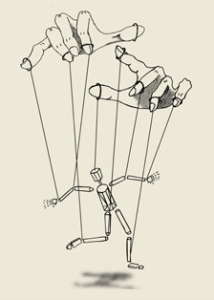
\includegraphics[height=2.5cm,width=2cm]{../pics/puppet.png}
\titlepage

\end{frame}

\begin{frame}

  \frametitle{Agenda}

  \begin{itemize}
  \item Was ist Puppet?
  \item Was ist Foreman?
  \item Puppet@s-iTSolutions
  \item Modul Entwicklung
  \item Deployment Prozess
  \end{itemize}

\end{frame}

\end{document}